
%%% Preamble
\documentclass[paper=a4, fontsize=11pt]{scrartcl}
\usepackage[T1]{fontenc}
%\usepackage{fourier}

\usepackage[english]{babel}															% English language/hyphenation
\usepackage[protrusion=true,expansion=true]{microtype}	
\usepackage{amsmath,amsfonts,amsthm} % Math packages
\usepackage[pdftex]{graphicx}	
\usepackage{url}
\usepackage{listings}
\usepackage{lmodern}


%%% Custom sectioning
%\usepackage{sectsty}
%\allsectionsfont{\centering \normalfont\scshape}


%%% Custom headers/footers (fancyhdr package)
\usepackage{fancyhdr}
\pagestyle{fancyplain}
\fancyhead{}											% No page header
\fancyfoot[L]{}											% Empty 
\fancyfoot[C]{}											% Empty
\fancyfoot[R]{\thepage}									% Pagenumbering
\renewcommand{\headrulewidth}{0pt}						% Remove header underlines
\renewcommand{\footrulewidth}{0pt}						% Remove footer underlines
\setlength{\headheight}{13.6pt}


%%% Equation and float numbering
\numberwithin{equation}{section}		% Equationnumbering: section.eq#
\numberwithin{figure}{section}			% Figurenumbering: section.fig#
\numberwithin{table}{section}			% Tablenumbering: section.tab#


%%% Maketitle metadata
\newcommand{\horrule}[1]{\rule{\linewidth}{#1}} 	% Horizontal rule

\title{
	%\vspace{-1in} 	
	\usefont{OT1}{bch}{b}{n}
	\normalfont \normalsize \textsc{University of Central Arkansas} \\ [25pt]
	\horrule{0.5pt} \\[0.4cm]
	\large Independent Study Report CRN: 31231 \\
	\huge Path Towards Caffeinated Deep Learning \\
	\horrule{2pt} \\[0.5cm]
}
\author{
	\normalfont 			\normalsize
	Abay Bektursun\\[-3pt]	\normalsize
	Fall 2017\\[-3pt]	\normalsize
}
\date{}



%%% Begin document
\begin{document}
	
	\maketitle
	\section{Fundamentals of Deep Learning}
		In this section I will shed some light onto the mathematical and computational concepts needed for understanding the basics of Deep Learning or any analytical methods for that matter. Most of the mathematical notation utilized here is same or similar to the one used in the famous "Deep Learning Book" [TODO: .bib]	
	
	\subsection{Challenges in Numerical Computation}
		Due to the limited nature of computer memory it is hard to store accurate representations of long real numbers. Therefore, we often approximate and round using floating points. This means that we will always have some errors when performing any useful numerical computations, even with higher precision floating points. Although there are numerical scientists who dedicate their careers to solving this kinds of problems, so we would not have to, it still important to be aware of the issues and challenges. 
	\paragraph{Overflow and Underflow.}
	There are cases where small rounding error can cause big problems in spite of the fact that approximations are often better than we even need them to be. For example, when a very small number is approximated to be zero. This problem is called Underflow. It's easy to imagine how things can go nuclear with Underflow: division by zero, or something along the lines of: $ \frac{1}{10^5}exp(95) $ will be zero if the fraction term is under approximated, but the true answer is about $ 10686.47458 $. Overflow is equivalently harmful problem. It occurs when a number with large absolute value is approximated to be $-\infty $ or $+\infty $. Consider the next: 
	\begin{align}
	softmax(x)_{i} = \frac{exp(x_{i})}{\sum_{j=1}^{n}exp(x_{j})}
	\end{align}
	This is Softmax function (1.1), it is often placed at the end of ANN topology. It is used to predict the probabilities associated with a multinoulli distribution. If all the values of $ x_{i} $ are equal to some arbitrarily large number, exponentiation will overflow, which in turn will lead to undefined answer. 
	\paragraph{Poor Conditioning}  
	The other common problem in numerical computing is poor conditioning. It refers to the problem of having large unexpected changes in the output of a function for small changes in the function's input. This kind of function with poor high condition is called ill-conditioned as oppose to well-conditioned problem.
	
	\subsection{Relevant Optimization Methods}
    In the heart of Machine Learning and therefore Deep Learning there lie mathematical optimization algorithms. The mathematical concepts behind most of the optimization methods existed for long time, but we were able to harness their power only in the recent past. The driving force behind Deep Learning is optimization algorithm called Backpropagation, which is concrete implementation of Gradient Descent (reviewed in the next subsections), and an application of the chain rule, the rule that was around since Leibniz times. There are few reasons why it took so long to come up with modern machine learning approaches, the obvious one being non-existence of practical computational power for most of the scientific history. Yoshua Bengio also has given a great answer on Quora to a question "Why did it take so long to invent the backpropagation algorithm?" [https://goo.gl/MT9mIo]. As he says: "Lots of apparently obvious ideas only became obvious after the fact..." I believe that theoretical work of pure mathematics have great potential that will drive the future Deep Learning algorithms and help us put together the first blue print of true intelligence.\par
    As the name suggest the main objective of a Deep Learning system is to learn, which is done through optimization. To have a clear understanding of what we are optimizing for, it is appropriate to use Mitchell's [1997] definition of learning: "A computer program is said to learn from experience E with respect to some class of tasks T and performance measure P, if its performance at tasks in T, as measured by P, improves with experience E." In supervised Deep Learning, performance measure P is the prediction accuracy of a system. Thus, our main objective is to maximize the P, concretely, to minimize the error of prediction. The main optimization approach used in Deep Learning is gradient based, and that is what we will be focusing on next.  
	\subsubsection{First-Order Optimization Algorithms}
    Given a function $ f(x) $, we need to minimize it by changing parameter $ x $ such that $ x* = arg\ min f(x)$. Superscript $*$ denotes a optimal value that optimizes $f(x)$. The function we are trying to optimize is called cost function, also known as objective function, loss function, criterion, and error function depending on literature and field. \par 
    First-Order optimization algorithm tries to minimize the cost function using its first order derivative $\frac{d}{dx}f(x)$ or shorter notation $f'(x)$. The main technique of doing so is Gradient Descent mentioned earlier. Derivative of a function tells us how the change in its input affects its output, and we could derive that for some input change $\epsilon $:\newline $f(x + \epsilon) \approx f(x) + \epsilon f'(x)$. It is also know that $ f(x - \epsilon sign(f'(x)) )  < f(x) $ given that $\epsilon$ is small enough. This is illustrated below (Fig 1.1). In the context of machine learning, $\epsilon$ is called learning rate, it is important hyperparameter for fine-tuning your learning system. \par
    
\begin{figure}[!htb]
	\centering
    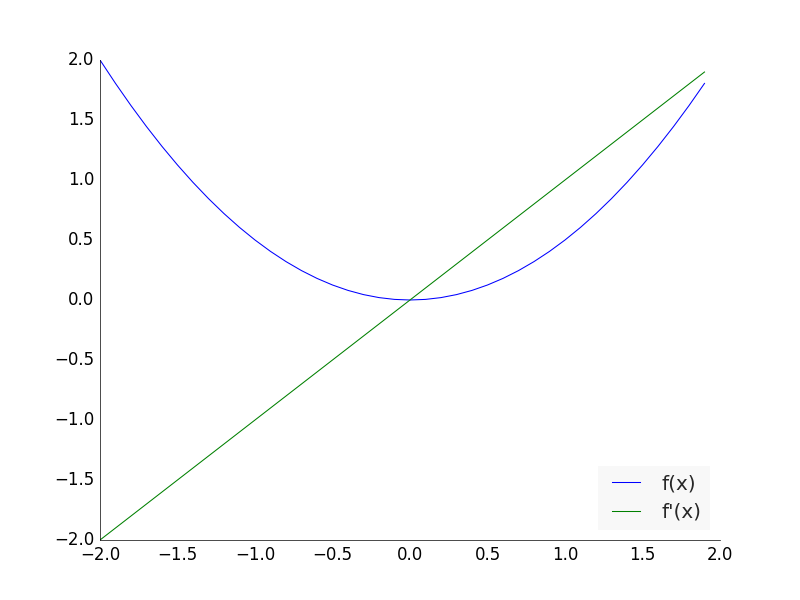
\includegraphics[scale=0.6]{gradient_descent.png}
    \caption{The blue line $ f(x) = \frac{1}{2}x^2$ and the green line $f'(x) = x $ visualize how we can arrive at the global minima of a convex function by shifting $x$ in with small enough $\epsilon$ sized steps towards opposite sign of the derivative of $f(x)$}
    \label{fig:fx_dfdx}
\end{figure}

Some terminology from Calculus:
\begin{itemize}
		\item Critical Points also known as Stationary Points are the points where $ f'(x) = 0 $ 
		\item Local Minima and Local Maxima is a point at some interval of $x$ where $f(x)$ is the smallest or largest respectively.
        \item Global Minima and Global Maxima are the absolute minimum or maximum point of $f(x)$ in all of $f(x)'s$ domain
        \item Saddle Points are the critical points that are neither any kind of maxima nor minima
	\end{itemize}
    It is unlikely that you will ever have a single variable cost function. Most Deep Learning problems train on image, video, and audio data sets. It is not rear that input of your system will be a hundred thousand dimensional vector. Therefore, we need to generalize gradient descent to $f: \mathbb{R}^n \rightarrow \mathbb{R} $. Notice that the output of the function is still scalar, this needs to be true in order to minimization objective to make sense. \par
    Instead of using derivative $\frac{d}{dx}f(x)$, we will need to use partial derivative, for example: $\frac{\partial}{\partial x_{i} }f(x)$ that tells us how output of $f(x)$ changes with respect to $x_{i}$ at point $x$, where $x_{i}$ is one of the variables in the input vector $x$. Gradient is an equivalent to the derivative in high dimensions. We write it as $\nabla_{x} f(x)$. Gradient is a vector consisting of all partial derivatives of $f(x)$. To find a critical point of high dimensional $f(x)$ is to find the gradient $\nabla_{x} f(x)$ of which all values are equal to zero. We could visualize a gradient using vector field. Here is an example with $\mathbb{R}^2$ gradient (Fig. 1.2).\par

\begin{figure}[!htb]
	\centering
    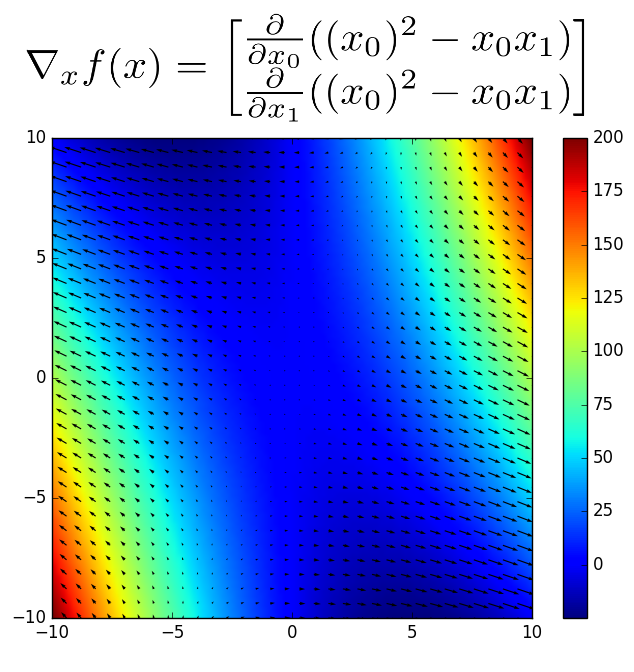
\includegraphics[scale=0.6]{Quiver_edited.png}
    \caption{Illustration of 2D  vector field where $x$-axis corresponds to the $x_0$ variable  and $y$-axis corresponds to $x_1$ variable. Here, you can see the area along the upward diagonal stripe in the middle of the vector filed where the arrows are very short. This area corresponds to $ x $ vectors where gradient gets closer and closer to zero}
    \label{fig:Quiver_gradient}
\end{figure}

 Now, we can actually talk about the main topic of this subsection, the steepest descent. The directional derivative in direction of unit vector $\vec{u}$ is slope of $f$ in direction $\vec{u}$. Directional derivative is formally defined as $$ \frac{\partial}{\partial \vec{u}} f(\vec{x}) = \lim_{h\to0} \frac{f(\vec{x} + h\vec{u}) - f(\vec{x})}{h} = \nabla_{\vec{v}} f(\vec{x})$$
We could look at one intuitive algebraic definition. Let say that we have a 2D vector $\vec{u} = \begin{bmatrix} a \\ b \end{bmatrix}$. Then our directional derivative of $f(\vec{x})$ in the direction of $\vec{u}$ is $a\frac{\partial}{\partial x_0}f + b\frac{\partial}{\partial x_1}f$. Notice that this is same as $\begin{bmatrix} a \\ b \end{bmatrix} \boldsymbol{\cdot} \begin{bmatrix} \frac{\partial f}{\partial x_0} \\  \frac{\partial f}{\partial x_1} \end{bmatrix} $ The second vector is the gradient so we can rewrite this as $\vec{u} \boldsymbol{\cdot} \nabla_{\vec{v}} f(\vec{x}) = \vec{u}^T \nabla_{\vec{v}} f(\vec{x}) $ This what we would get if we derived from the formal definition using chain rule.  \par
So we would like to find direction in which $f$ decreases fastest, or we would like to minimize $f$. We do it making use of directional derivative 
$$\underset{u,u^Tu=1}{\text{min}} u^T\nabla_x f(x) =$$
$$ = \underset{u,u^Tu=1}{\text{min}} ||u||_2||\nabla_x f(x)||_2cos(\theta) $$


	\subsubsection{Second-order Optimization Algorithms}
	The optimization methods that involve second order derivatives are called Second-order. There are some advantages of Second-order Optimization Algorithms, but unfortunately they do not always work, if at all. The example of such algorithm would be one that uses Newton's method to jump the desired optima. 
	
	\subsection{Probability}
	\subsection{Neural Networks}
	\subsubsection{Feedforward Example}
	It's a good idea to walk thorough example of a feed forward network. The most common example shown in introductory Deep Learning courses is learning XOR (exclusive 'or') function. XOR takes in two binary values and returns 1 if only one of the two variables is equal to 1, returns 0 otherwise. 
	Let $X$ be our design matrix that consists of all the possible input vectors. Let $y$ be the corresponding outputs. 
		$$ X = 
		\begin{bmatrix}
			0 & 0 \\
			0 & 1 \\
			1 & 0 \\
			1 & 1
		\end{bmatrix} 
		y = 
		\begin{bmatrix}
		0 \\
		1 \\
		1 \\
		0 
		\end{bmatrix}$$
	We set our cost function to me a mean squared error $J(\theta)$ just for this example. The Deep Learning book describes more appropriate functions for binary input [cite], but for simplicity sake using MSE would be appropriate:
		$$ J(\theta)=\frac{1}{4}\sum_{x\in X}^{}(y-f(x;\theta))^2 $$
	
	\begin{figure}[!htb]
		\centering
		\includegraphics[scale=0.6]{xor_ex.png}
		\caption{Visualization of the Caffe architecture used to train the Cifar models}
		\label{fig:cifar}
	\end{figure}
	
	
	
	\section{Introduction to Caffe}
	Caffe is a one of the few industry strength Deep Learning Frameworks. It is an open-source software created by The Berkeley Artificial Intelligence Research (BAIR) Lab that started out as Yangqing Jia's thesis who was UC Berkeley's PhD student at that time [http://daggerfs.com/]. The strength of Caffe is its performance and ease of use. According to its developers it was made with expression, speed, and modularity in mind. It's main weakness is flexibility, or absence of it. Architecture in Caffe is defined in protobuff format using predefined nodes and optimization algorithms, leaving the developer to arrange the nodes and tune hyperparameters. Caffe has been most widely used Deep Learning framework both in Academia and Industry, although that title has slipped to TensorFlow's ownership in the recent past. Even the original developer Yangqing Jia moved on to help developing TensorFlow. Seeing the rise of projects like TensorFlow, Torch, and Theano, it seems like Caffe will not be one of the leading frameworks of the future. Nevertheless, Caffe will have its place a great prototyping tool and solution for time constrained agile projects. Caffe has it's own philosophy [http://caffe.berkeleyvision.org]:
		\begin{itemize}
			\item Expression: models and optimizations are defined as plaintext schemas instead of code.
			\item Speed: for research and industry alike speed is crucial for state-of-the-art models and massive data. 
			\item Modularity: new tasks and settings require flexibility and extension.
			\item Openness: scientific and applied progress call for common code, reference models, and reproducibility.
			\item Community: academic research, startup prototypes, and industrial applications all share strength by joint discussion and development in a BSD-2 project.
		\end{itemize}
	
	\section{Training Convolutional Neural Network on Caffe}
	\begin{figure}[!htb]
		\centering
		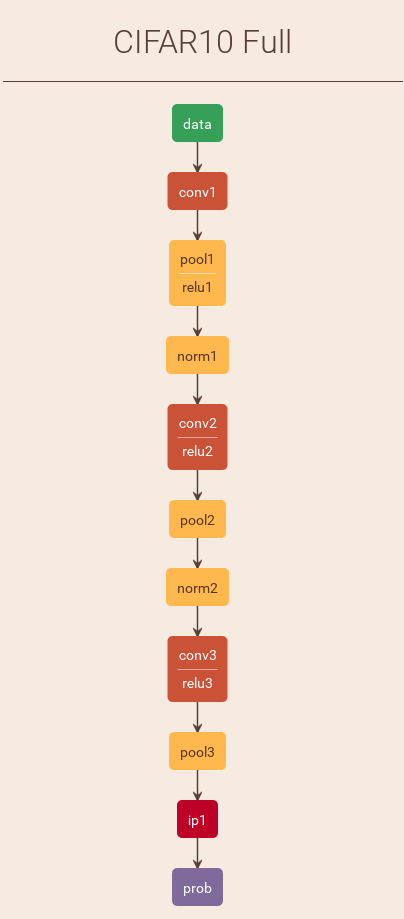
\includegraphics[scale=0.4]{cifar.png}
		\caption{Visualization of the Caffe architecture used to train the Cifar models}
		\label{fig:cifar}
	\end{figure}

	There first 'data' layer is defined by a data node that takes in mdb data input (Caffe understandable data format) with shape (channels and size):
	\begin{lstlisting}[language=xml]
	{ dim: 1 dim: 3 dim: 32 dim: 32 }
	\end{lstlisting}
	By froward pass path, data layer is fed to 'conv1' which is defined as five filters with stride of one.
	
	
	\section{Testing and Tuning Hyperparameters}
	Here, model was trained on CIFAR-10 dataset that is consists of 60000 image with 3 color (RGB) channels and 32x32 pixels. The whole dataset is around 160Mb and has 10 independent classes with 6000 images for each. It is split into training and testing sets with 50000 and 10000 images in each respectively. 
	
	The highest score obtained in this example of course are not as good as state of the art object recognition results, since the training images are not always fair:
	\begin{figure}[!htb]
		\centering
		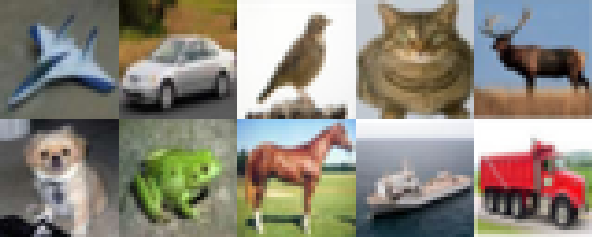
\includegraphics[scale=1.0]{cifar10.png}
		\caption{There are many images that do not carry information needed due to low resolution. Often predicting the class of an object is even hard for humans}
		\label{fig:cifar10ex}
	\end{figure}
	\newline Here is are descriptions of the system used for training: 
	\begin{verbatim}
	
	H/W path                Device      Class       Description
	=============================================================================
	system      To Be Filled By O.E.M. (To Be Filled By O.E.M.)
	/0/4/5                              memory      288KiB L1 cache
	/0/4/6                              memory      6MiB L2 cache
	/0/4/7                              memory      8MiB L3 cache
	/0/e                                memory      8GiB System Memory
	/0/100/2/0                          display     GM206 [GeForce GTX 960]
	\end{verbatim}
	Full:      
		61m 58.334s
	Test net output: accuracy = 0.8148
	\newline Quick: 
		0m 50.972s
	Test net output: accuracy = 0.7535
	
	
	
	
	\section{Analysis of the Results and Further Investigation of Conv Net Architectures}
	\section{Classification of Skin Cancer Using GPU Accelerated [Architecture] on Caffe}
	\section{Analysis of the Skin Cancer Classification Results}
	
	

\bibliographystyle{plain}
\bibliography{ref}


\end{document}
